%%%%%%%%%%% INCLUSÃO DE PACOTES %%%%%%%%%%%%%%%%
% Classe Base do Documento: Artigo
\documentclass [12pt]{article}
% Layout do Papel
\usepackage{Layout/Layout_Documento}
% Case não funcione, verificar o diretório do arquivo 'Layout_Documento.sty'
%\usepackage{lipsum}
%%%%%%%%%%% FIM INCLUSÃO DE PACOTES %%%%%%%%%%%

%%%%%%%%%%% INFORMAÇÕES BÁSICAS %%%%%%%%%%%%%%%
\title {Projeto Final BD}
%%%%%%%%%%% FIM INFORMAÇÕES BÁSICAS %%%%%%%%%%%

\begin{document}
	\inserirTitulo
	
	\section{Introdução}
		\label{sec:intro}
	Quando há requisito de eficiência nas organizações, tanto com fins lucrativos ou não, é importante que haja conhecimento sobre os dados que transitam por tal organização. Tais dados devem ser trabalhados de modo a se adquirir informações úteis para um bom planejamento, do gerencial ao estratégico.
	
	É possível armazenar tais dados em memória simples de um computador, sendo esta um HD, e realizar todas as operações sobre tais dados; mas há o caso de que, cada vez mais, a massa de dados vem aumentado. Tal aumento exige um gerenciamento adequado, promovido pelos~\emph{Sistemas Gerenciadores de Banco de Dados} (\emph{SGBDs}).
	
	Primeiramente, é preciso compreender o que seria um~\emph{banco de dados} (BD): pode ser visto como o equivalente eletrônico de um armário de arquivamento, uma vez que é a coleção de dados persistentes utilizadas pelos sistemas de aplicação de uma empresa. Dessa forma, um SGBD é responsável pelo gerenciamento dessas coleções, garantindo integridade, segurança e outras características.

	Os dados podem ser extraídos de qualquer fonte, mas, para este trabalho, será utilizada a~\emph{INDA} (\emph{Infraestrutura Nacional de Dados Abertos}); visto que são dados que estão à disposição livremente a todos, mas apenas alguns a acessam. Dessa forma, ao se trabalhar com tais dados e gerar informações consideráveis estaríamos exercendo a nossa cidadania, buscando discrepâncias entre os dados e apontando algumas irregularidades.
	
	Como escopo, foi escolhido os dados sobre~\textbf{Diárias e passagens}~(Tais dados estão disponível~\emph{online}: \url{http://www.portaltransparencia.gov.br/}) limitados ao período: $jan/2015$ a $jun/2015$, visando responder os seguintes questionamentos:
	
	\begin{enumerate}
		\item Qual o gasto total em cada mês?
		\item Quais os órgãos que mais gastaram?
		\item Quais os programas que mais gastaram?
		\item Quais os servidores que mais gastaram?
		\item Quais as funções que mais gastaram?
	\end{enumerate}

	\section{Diagrama Entidade Relacionamento (DER)}
		\label{sec:DER}
	Um DER constitui uma forma de representação gráfica para os conceitos atribuídos ao~\emph{Modelo Entidade Relacionamento} (MER), sendo este um modelo de dados conceitual de auto nível, visto que está centrado na percepção dos usuários sobre os dados, não importando a maneira na qual os dados serão armazenados. Dessa forma, entendisse DER como representação visual sobre os dados que serão tratados no BD.
		
	Como os dados fornecidos vem em forma de planilhas, foi preciso realizar uma leitura e uma interpretação dos mesmos, tentando identificar o que veriam a ser as entidades e os relacionamentos para o nosso BD. Dessa forma, obteve-se a Figura~\ref{fig:DERgerado} como resutaldo do estudo realizado.
	
	\begin{figure}[h]
		\centering
		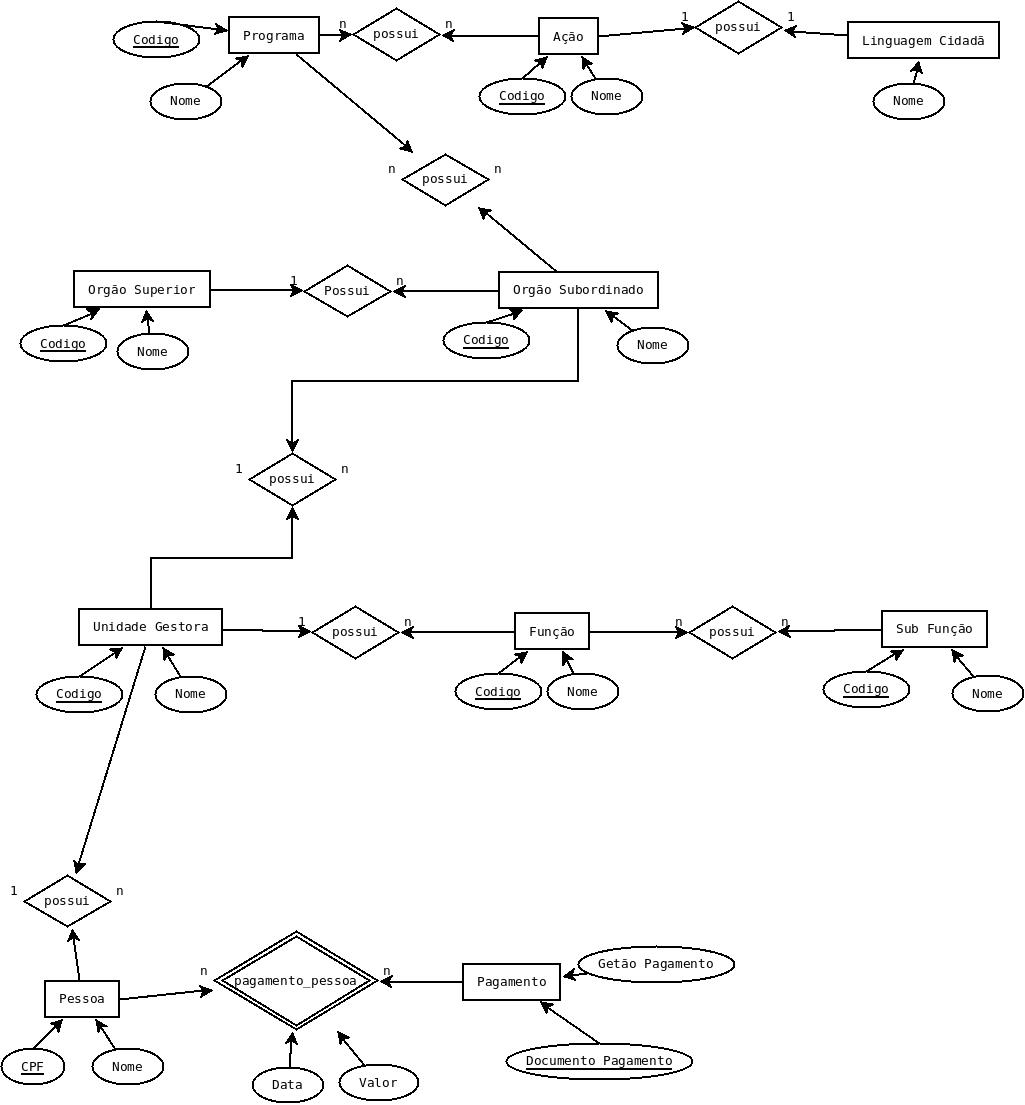
\includegraphics[width=1\textwidth]{Imagens/DER}
		\caption{DER gerado a partir das tabelas e nossa interpretação.}
		\label{fig:DERgerado}
	\end{figure}
	
	
	\section{Modelo Relacional (MR)}
		\label{sec:MR}
	Um MR representa os dados num BD como uma coleção de relações, denominadas de tabelas. Essa coleção será implantada no SGBD, ou seja, o MR representa a construção física do BD. Por isso é desenvolvido a partir do DER e, no escopo deste trabalho, tem-se a Figura~\ref{fig:MRgerado} como resultado.
	
	\begin{figure}[h]
		\centering
		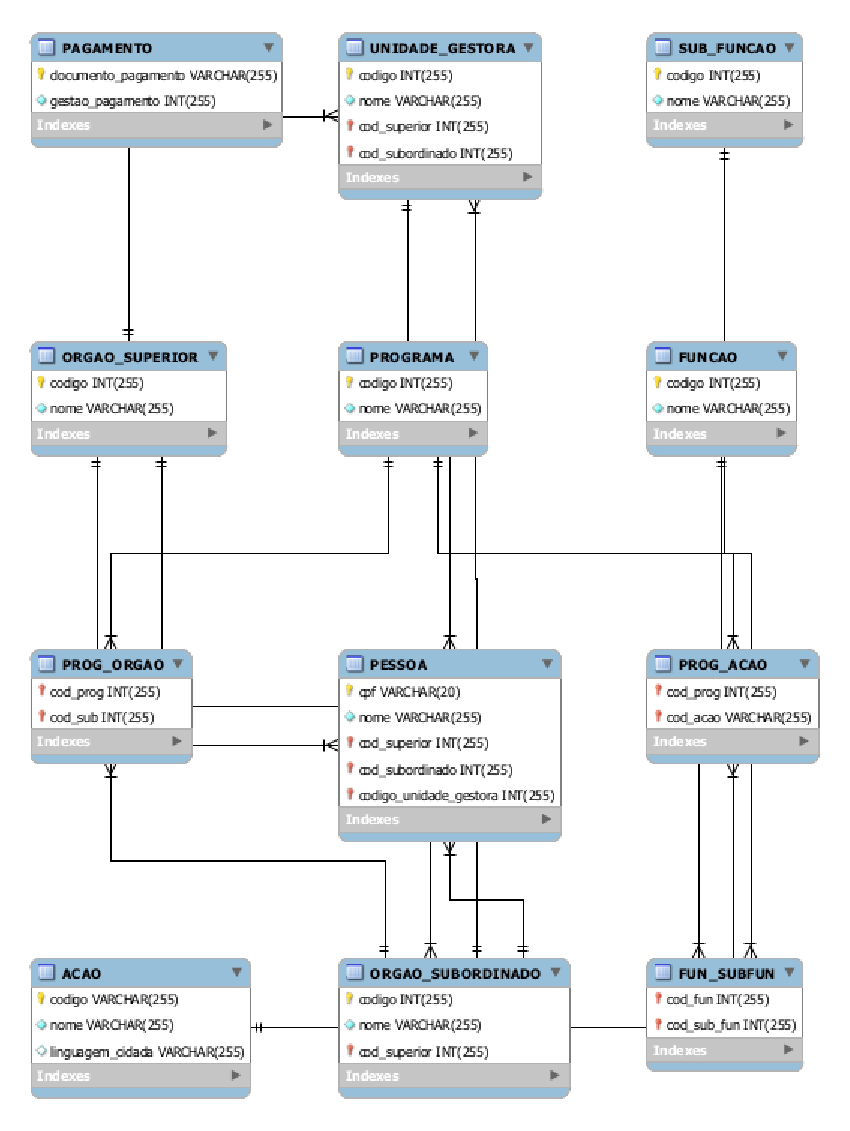
\includegraphics[width=.8\textwidth]{Imagens/MR}
		\caption{MR gerado a partir do DER.}
		\label{fig:MRgerado}
	\end{figure}
	
	\section{Avaliação das formas normais}
		\label{sec:FormaisNormais}
	A normalização é importante para identificar um bom projeto relacional. Um bom MER e sua consequente conversão para um MR, praticamente, deixa o esquema relacional~\emph{normalizado}	.
	
	Ao se tratar de normalização, consideram-se três formais normais, onde: na primeira (1FN) há a caracterização de um valor de uma coluna de uma tabela é indivísel; na segunda (2FN), se estiver na 1FN e todo atributo do complemento de uma chave candidata é totalmente funcionalmente dependente daquela chave; for fim, na terceira, se estiver na 2FN e todos os atributos não-chave forem dependentes não-transitivos da chave primária.
	
	Dessa forma, foram selecionadas três tabelas: Pessoa, Ação e Função; onde:
	
	\newpage
	\begin{itemize}
		\item \textbf{Pessoa:}
			\begin{table}[h]
				\centering
				\begin{tabular}{|c|c|c|c|c|} \hline
					{\ul Cpf} & Nome & Cod\_superior & Cod\_subordinado & Cod\_unidade\_gestora \\ \hline
				\end{tabular}
			\end{table}
			
			\begin{itemize}
				\item 1FN: Todos os valores das colunas da tabela são indivisíveis;
				\item 2FN: Chave candidata: Cpf
					\begin{eqnarray*}
						Cpf & \rightarrow & Nome \\
						Cpf & \rightarrow & Cod\_superior \\
						Cpf & \rightarrow & Cod\_subordinado \\
						Cpf & \rightarrow & Cod\_unidade\_gestora
					\end{eqnarray*}
				\item 3FN: Não há nenhuma transitividade nas colunas, uma vez que todos são definidos unicamente somente pelo Cpf.
			\end{itemize}
			
		\item \textbf{Ação:}
			\begin{table}[h]
				\centering
				\begin{tabular}{|c|c|c|} \hline
					{\ul Codigo} & Nome & Linguagem\_cidada \\ \hline
				\end{tabular}
			\end{table}
			
			\begin{itemize}
				\item 1FN: Todos os valores das colunas da tabela são indivisíveis;
				\item 2FN: Chave candidata: Código
					\begin{eqnarray*}
						Codigo & \rightarrow & Nome \\
						Codigo & \rightarrow & Linguagem\_cidada
					\end{eqnarray*}
				\item 3FN: Não há nenhuma transitividade nas colunas, uma vez que todos são definidos unicamente somente pelo Código.
			\end{itemize}
			
		\item \textbf{Função:}
			\begin{table}[h]
				\centering
				\begin{tabular}{|c|c|} \hline
					{\ul Codigo} & Nome \\ \hline
				\end{tabular}
			\end{table}
			
			\begin{itemize}
				\item 1FN: Todos os valores das colunas da tabela são indivisíveis;
				\item 2FN: Chave candidata: Código
					\begin{eqnarray*}
						Codigo & \rightarrow & Nome
					\end{eqnarray*}
				\item 3FN: Não há nenhuma transitividade nas colunas, uma vez que todos são definidos unicamente somente pelo Código.
			\end{itemize}
	\end{itemize}
		
	\section{Criação do BD}
		\label{sec:BDcreate}
	A partir do MR construído, foi realizado o processo da engenhaia reversa, de modo a ser obter o~\emph{script} corresponde à criação daquele BD. Como resultado tem-se, para apenas uma tabela, o~\emph{script} demonstrado no Listing 1.
	
	\lstinputlisting[caption = Trecho referente à criação do BD e de uma tabela no MySQL.]
					{Documentos/criarBanco.sql}
		
	\section{Processo de ETL}
		\label{sec:ETL}
	Como já foi anteriormente na Seção~\ref{sec:DER}, os dados obtidos a partir da INDA são planilhas e para elas é preciso realizar um processo, de forma a se obter dados interpretáveis pelo SGBD utilizado, que no caso foi o~\emph{MySQL Workbench}. Tal processo é denominado~\emph{Processo ETL} (\emph{Extract}, \emph{Transform}, \emph{Load}), pois nele há a extração dos dados existentes nas planilhas, há uma manipulação para formatar a inserção no SGBD e, por fim, há o povoamento do BD com os dados extraídos das planilhas.
	
	As primeiras duas etapas do processo foram realizadas por um programa me linguagem JAVA, enquanto que a última era realizada diretamente no SGBD. Como resultado da primeira parte há um \emph{script} .sql com todas as inserções, tal \emph{script} é executado na segunda parte.

	Todas as planilhas tem os mesmos tipos de dados e nas mesmas colunas, num total de $21$ colunas. Com este conhecimento e sabendo o MR, que deveria ser implementado, a extração ocorreu de forma a respeitar tais conhecimento e os relacionados à Seção~\ref{sec:FormaisNormais}, tendo os atribuitos-chave únicos para cada registro. Na etapa de transformação, há a formação do comando de inserção, que segue a sintaxe do Listing 2.
	
	\lstinputlisting[caption = Trecho referente à sintaxe de inserção no MySQL.
					\label{lis:insert}]
					{Documentos/insert.sql}
	
	\section{Persistência e Visualização}
		\label{sec:Per&Vis}
	A camada de persistência e o ambiente para visualização dos dados foram feitos com a plataforma~\emph{OutSystems} e está disponível no endereço:~\url{https://diegoleite.outsystemscloud.com/Trab_BD/}
	
	\section{View, Procedure e Trigger}
		\label{sec:VPT}
	As~\emph{view} são tabelas virtuais criadas a partir de um~\emph{SELECT}. Normalmente, são utilizadas para prover segurança e facilidade de desenvolvimento. As~\emph{procedure} são programas que podem ser armazenados no SGBD, onde cada SGBD tem suas próprias linguagens. E as~\emph{triggers} é um objeto de banco de dados, associado a uma tabela, definido para ser disparado, respondendo a um evento em participar.
	
	Dessa forma foram desenvolvidas os seguintes arquivos.
	
	\lstinputlisting[caption = Trecho referente à~\emph{view} desenvolvida.
					\label{lis:insert}]
					{Documentos/view.sql}
					
	\lstinputlisting[caption = Trecho referente ao~\emph{procedure} desenvolvido.
					\label{lis:insert}]
					{Documentos/procedure.sql}
	
	\lstinputlisting[caption = Trecho referente ao~\emph{trigger} desenvolvido.
					\label{lis:insert}]
					{Documentos/trigger.sql}
\end{document}
